\chapter{Waves}
	\section{Fundamentals of Waves} \index{Wave}

	You have probably heard of waves in the context of the ocean, a lake, or other bodies of liquid.  Waves are also found in earthquakes, sound, light, and even at the stadium when people do ``the wave.''  A \textit{wave} is a distortion that transfers energy from one place to another without the permanent transfer of mass. 
	
	The material that a wave travels through is called a \textit{medium}. \index{Medium} \index{Wave, medium} For instance, the medium for an ocean wave is water, while the medium for light could be air, glass, water, or even empty space (no medium).  

		\subsection{Types of Waves}
	 Waves can be categorized into several basic types: 
	\begin{itemize}
		\item \textit{Transverse Waves} - are waves that are displaced perpendicular to the direction of travel.  For instance, ocean waves are a type of transverse wave because their displacement is vertical, though they travel horizontally.
		Normally, a transverse wave is drawn similar to the figure below:
		\begin{center}
		\begin{figure}[h]
			\centering
			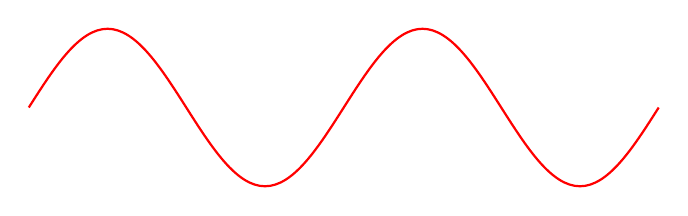
\begin{tikzpicture}

				 \draw[thick, red]
				 (3,0) sin (4,1) cos (5,0) sin (6,-1) cos (7,0)
				 sin (8,1) cos (9,0) sin (10,-1) cos (11,0);	
			 \end{tikzpicture}
			 \caption{A simple transverse wave}
		\end{figure}
		\end{center}	
		
		\item \textit{Longitudinal Waves} - are waves that are displaced in the same direction as the direction of travel.  You can think of this as a compression, or shock wave that travels through a medium.  The places where a material is closer together than normal are called compressions, while places that are spaced farther apart are called rarefractions, as seen in figure \ref{tester}
		
		\begin{figure}[h]
			\centering
			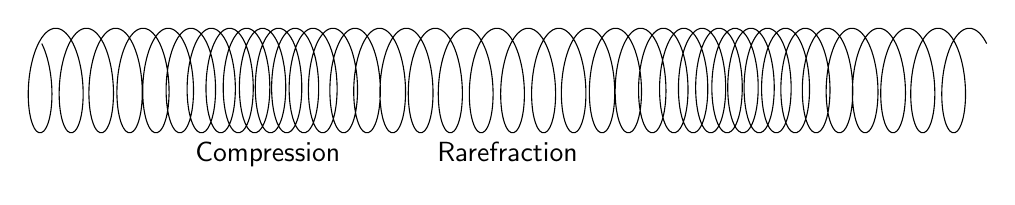
\begin{tikzpicture}[font=\sffamily] 
			\begin{scope}[z={(70:1)},y={(110:1)},local bounding box=coil] 
			\draw plot[domain=0:14400,variable=\t,samples=1441,smooth] 
			({\t/1200+0.1*pi*sin(\t/20)},{-0.5*sin(\t)},{0.5*cos(\t)}); 
			\end{scope} 
			\path (coil.south west) -- (coil.south east) 
			node[pos=0.25,below]{Compression} node[pos=0.5,below]{Rarefraction}; 
			
		\end{tikzpicture} 


			
			\caption{A simple longitudinal wave}
			\label{tester}
		\end{figure}	
		
		\item \textit{Electromagnetic Waves} - are waves that are made up of oscillating electric and magnetic fields.  These are usually modeled as transverse waves, but they are just representations of the strength of the electric and magnetic fields. 
		
		
		\begin{figure}[h]
			\centering
			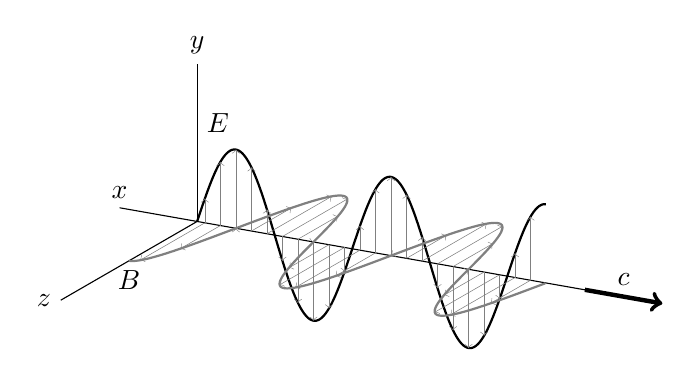
\begin{tikzpicture}[x={(-10:1cm)},y={(90:1cm)},z={(210:1cm)}]
			% Axes
			\draw (-1,0,0) node[above] {$x$} -- (5,0,0);
			\draw (0,0,0) -- (0,2,0) node[above] {$y$};
			\draw (0,0,0) -- (0,0,2) node[left] {$z$};
			% Propagation
			\draw[->,ultra thick] (5,0,0) -- node[above] {$c$} (6,0,0);
			% Waves
			\draw[thick] plot[domain=0:4.5,samples=200] (\x,{sin(deg(pi*\x))},0);
			\draw[gray,thick] plot[domain=0:4.5,samples=200] (\x,0,{cos(deg(pi*\x))});
			% Arrows
			\foreach \x in {0.1,0.3,...,4.4} {
				\draw[->,help lines] (\x,0,0) -- (\x,{sin(deg(pi*\x))},0);
				\draw[->,help lines] (\x,0,0) -- (\x,0,{cos(deg(pi*\x))});
			}
			% Labels
			\node[above right] at (0,1,0) {$\bm{E}$};
			\node[below] at (0,0,1) {$\bm{B}$};
			\end{tikzpicture}	
			\caption{An electromagnetic wave}
		\end{figure}
		 
		Electromagnetic waves are what make up the electromagnetic spectrum.  Radio waves, microwaves, infrared, visible light, ultraviolet, X-rays and $\gamma$-rays are all electromagnetic waves.  They are categorized into different types based on their frequency. 
		 
	\end{itemize}

	There are other types of waves, such as matter waves and gravitational waves that are beyond the scope of this text.  

\newpage
		\subsection{Basic Wave Characteristics and Vocabulary}
		
\begin{center}
	\begin{figure}[h]
		\centering
		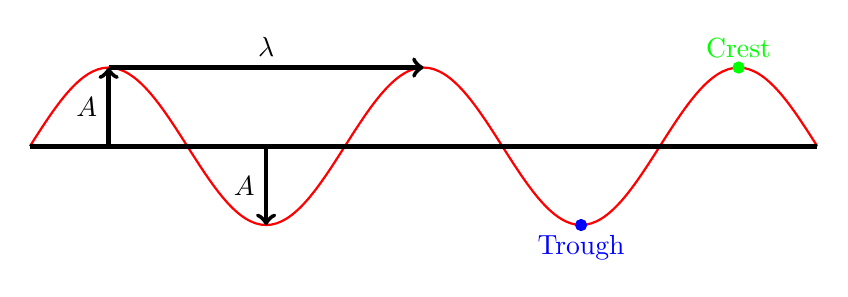
\begin{tikzpicture}
		
		\draw[thick, red]
		(3,0) sin (4,1) cos (5,0) sin (6,-1) cos (7,0)
		sin (8,1) cos (9,0) sin (10,-1) cos (11,0) sin (12,1) cos (13,0);	
			\draw[-,ultra thick] (3,0) --  (13,0);
			\draw[->,ultra thick] (4,1) -- node[above] {$\lambda$} (8,1);
			\draw[->,ultra thick] (4,0) -- node[left] {$A$} (4,1);
			\draw[->,ultra thick] (6,0) -- node[left] {$A$} (6,-1);
		 	\draw [blue] (10,-1) circle[radius=2pt] node[below] {Trough};
		 	\fill[blue] (10,-1)  circle[radius=2pt];
	 		\draw [green] (12,1) circle[radius=2pt] node[above] {Crest};
		 	\fill[green] (12,1)  circle[radius=2pt];
		 	
		\end{tikzpicture}
		\caption{The measurements of a wave}
		\label{fig:wavemeasure}
	\end{figure}
\end{center}	
		
	\subsubsection{Extrema} \index{Crest} \index{Trough} \index{Wave, Crest} \index{Wave, Trough} 
	
	\textbf{Crests} are each of the highest points of a wave, and \textbf{troughs} (rhymes with coughs) are the lowest points of a wave, as seen in the diagram \ref{fig:wavemeasure}.  The word \textbf{extrema} refers to all crests and troughs, as they are the most extreme points of the wave. 
	
	\subsubsection{Amplitude} \index{Amplitude} \index{Wave, Amplitude} \textbf{Amplitude} measures how large or how strong a wave is.  It is measured from the center of a wave to one of the extrema - either upward to a crest, or downward to a trough.  For a physical, transverse wave, amplitude can be measured in meters.  The variable for amplitude is $A$.  For sound, we experience the amplitude of the wave as \textit{volume}, and for light, we experience it as \textit{brightness}.
	
	\subsubsection{Wavelength} \index{Wavelength}
	The \textbf{wavelength} of a wave is measured from any point to an identical point on the wave, along the axis of propagation.  Wavelength is measured in meters, and the symbol for wavelength is $\lambda$ (lambda).  The easiest way to measure wavelength is from crest to crest or from trough to trough. 
	
	\subsubsection{Period} \index{Period} \index{Wave, Period}
	The \textbf{period} of a wave measures how long it takes a wave to repeat itself.  It is measured in seconds, and uses the variable $T$.  
	
	\subsubsection{Frequency} \index{Frequency} \index{Wave, Frequency}
	The \textbf{frequency} of a wave measures how many times a wave repeats itself in one second.  The symbol for frequency is $f$ and the units for frequency are $\frac{cycles}{second} $.  We give this unit the name \textit{hertz}, abbreviated Hz. For sound, we experience frequency as \textit{pitch}, and for light we experience frequency as \textit{color}. 
	
	\newpage
	
	The frequency of a wave and the period of a wave are inverses of each other.  Thus:
	
	
	\begin{mdframed}[backgroundcolor=orange!20!white]
		\begin{equation}
		f = \frac{1}{T}
		\label{equation:wavefrequency}
		\end{equation}
	\end{mdframed}	
	
	
	
	\begin{mdframed}[backgroundcolor=blue!10!white]
		\begin{center}
			
			
			\textbf{Example \thesection.1}	
		\end{center}
		
		\textbf{Problem: }A wave has a frequency of 102.1 MHz.  What is the period of the wave?
		\vspace{0.1in}
		
		\textbf{Solution:} 
		
		We know that $f = \SI{102.1}{\mega\hertz} $ Converting into scientific notation gives:
		 
		 	
		 \begin{equation*}
		 f = \SI{102.1}{\mega\hertz} = \SI{102.1e6}{\hertz} = \boxed{ \SI{1.021e8}{\hertz}}
		 \end{equation*}
		 
		
		Begin by using equation \ref{equation:wavefrequency}:
		
		
		\begin{equation*}
		f = \frac{1}{T}
		\end{equation*}
		
		Solving for $T$ yields:
		
		\begin{equation*}
			T = \frac{1}{f}
		\end{equation*}		
		
		Then, substitute numbers: 
		
		\begin{equation*}
		T = \frac{1}{\SI{1.021e8}{\hertz}} \approx \boxed{\SI{9.794e-9}{\s}}
		\end{equation*}		
		
	\end{mdframed}
	
	\subsection{Velocity of a Wave} \index{Velocity of a Wave} \index{Wave, Velocity}
	
	We already know from equation \ref{eqn:velocity} that the average velocity of any object is given by $\overrightarrow{v_{avg}} = \frac{\vec{d}}{\Delta t} $.  In the case of a wave, the time it takes the wave to repeat is the period, $T$, and distance the wave must move in order to repeat is one wavelength, $\lambda$.  Thus, $\overrightarrow{v_{avg}} = \frac{\vec{d}}{\Delta t} = \frac{\vec{\lambda}}{T}$.  Using equation \ref{equation:wavefrequency}, it can be proven that:
	
		\begin{mdframed}[backgroundcolor=orange!20!white]
		\begin{equation}
		v = f\lambda
		\label{equation:wavevelocity}
		\end{equation}
	\end{mdframed}	
	
	
	\newpage
	
	\begin{mdframed}[backgroundcolor=blue!10!white]
	\begin{center}
		
		
		\textbf{Example \thesection.2}	
	\end{center}
	
	\textbf{Problem: }An ocean wave has a period of 15 seconds, and is traveling at a speed of 2 meters per second.  How far is it from one crest of the wave to another? 
	
	\vspace{0.1in}
	
	\textbf{Solution:} 
	The question asks for the distance from one crest to another, which is the wavelength.  
	Given values:  \begin{center}
					$T = \SI{15}{\s}$

					$v = \SI[per-mode = symbol]{2}{\m\per\s} $
					\end{center}

	First, we use equation \ref{equation:wavefrequency} to find the frequency:
		\begin{equation*}
	f = \frac{1}{T} = \frac{1}{\SI{15}{s}} \approx \SI{0.067}{\s}
	\end{equation*}

	We now use equation \ref{equation:wavevelocity}:
	\begin{equation*}
		v = f\lambda
	\end{equation*}
	
	Solving for wavelength gives:
		\begin{equation*}
	\frac{v}{f} = \lambda
	\end{equation*}
	
	Substituting gives: 
	
	
	\begin{equation*}
	\lambda = \frac{v}{f} \approx \frac{\SI[per-mode = symbol]{2}{\m\per\s}}{\SI{.067}{\s}} \approx \boxed{\SI{30}{\m}}
	\end{equation*}		
	
\end{mdframed}
	
		
	
	\newpage
	
	
\section{The Doppler Effect} \index{Doppler Effect}
	We have all experienced a car driving past us while it is honking its horn.  As the car drives past, there is a significant change in the pitch of the horn.  In fact, when either the source of a wave or an observer of a wave is moving, it causes the observer's perception of the frequency of that wave to change.  This is called the \textbf{Doppler Effect}.  
	
	When the source of a wave moves \textit{toward} an observer, its frequency is shifted higher.  
	
	\begin{figure}[h]
		\centering
		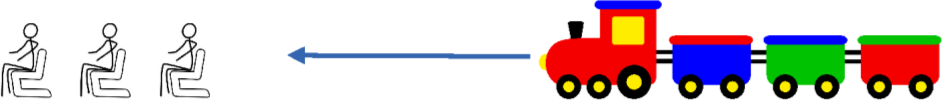
\includegraphics[height=0.3in,width=4in]{Chapters/Ch10-Waves/Doppler1.png}
		\caption{Observers hear a higher pitch}
	\end{figure}
	
	When the source of a wave moves \textit{away} from an observer, its frequency is shifted lower.  
	
		
	\begin{figure}[h]
		\centering
		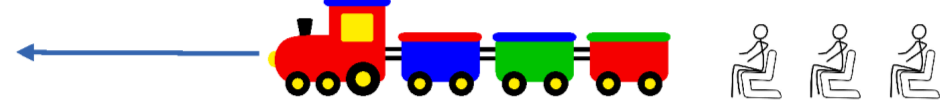
\includegraphics[height=0.3in,width=4in]{Chapters/Ch10-Waves/Doppler2.png}
		\caption{Observers hear a lower pitch}
	\end{figure}
	
	Likewise, when an observer moves \textit{toward} the source of a sound, its frequency is shifted higher.
	
			
	\begin{figure}[h]
		\centering
		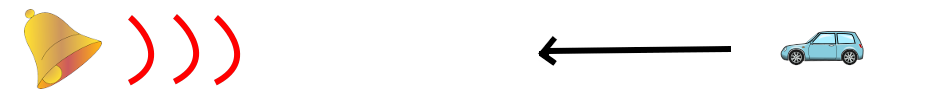
\includegraphics[height=0.3in,width=4in]{Chapters/Ch10-Waves/Doppler3.png}
		\caption{Observer hears a higher pitch}
	\end{figure}
	
	
	
	When an observer moves \textit{away} from a source of sound, its frequency is shifted lower.   
	
	
				
	\begin{figure}[!h]
		\centering
		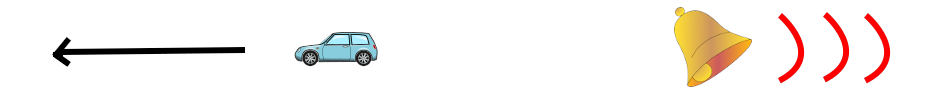
\includegraphics[height=0.3in,width=4in]{Chapters/Ch10-Waves/Doppler4.png}
		\caption{Observer hears a lower pitch}
	\end{figure}
	
	

	
	The equation for the Doppler effect is given by equation \ref{equation:dopplereffect}:
	
	

	
	
	
		\begin{mdframed}[backgroundcolor=orange!20!white]
		\begin{equation}
		f_{observed} = f_{source}(\frac{v_{wave} \pm v_{observer}}{v_{wave} \pm v_{source}})
		\label{equation:dopplereffect}
		\end{equation}
	\end{mdframed}	
	
		

	
	In this equation, do not consider the $\pm$ sign to represent both operations.  Instead, you must chose which operation to use based on the given situation.  In the numerator of the equation it is exactly what is expected: add for a higher frequency and subtract for a lower frequency.  In the denominator, it is backward - add for lower frequency, and subtract for higher frequency.  
	
	
	
	In the air, the speed of sound depends on air pressure, temperature, and even humidity.  The standard value for speed of sound in air is \textbf{343 m/s}, though in reality this number can change quite significantly depending on atmospheric conditions.  
	
		\newpage
	
	
	
	
	
	
	\begin{mdframed}[backgroundcolor=blue!10!white]
	\begin{center}
		
		
		\textbf{Example \thesection.1}	
	\end{center}
	
	\textbf{Problem: } A car's horn has a pitch of 550 Hz.  It is driving at 15 m/s toward a stationary observer.  \begin{enumerate}
		\item[a.] What is the frequency that the observer hears at the car approaches. 
		\item[b.] The car then passes the observer.  What is the frequency that the observer hears as the car travels away from him?  
		
	\end{enumerate}
	
	\vspace{0.1in}
	
	\textbf{Solution:} A car's horn produces sound, therefore the velocity of the wave is the speed of sound. 
  
	\underline{Part a:} Given values:  \begin{center}
		$f_{source} = \SI{550}{\Hz}$
		
		$v = \SI[per-mode = symbol]{343}{\m\per\s} $
		
		$v_{source} = \SI[per-mode = symbol]{15}{\m\per\s} $
		
		$v_{observer} = \SI[per-mode = symbol]{0}{\m\per\s} $
	\end{center}
	
	We can use equation \ref{equation:dopplereffect} to find the frequency the observer hears:

	\begin{equation*}
			f_{observed} = f_{source}(\frac{v_{wave} \pm v_{observer}}{v_{wave} \pm v_{source}})
	\end{equation*}
	
	In this case, the observer is not moving, so it does not matter whether we chose a plus or minus.  The source is moving toward the observer, causing the observer to hear a higher pitch.  Therefore, since the source is in the denominator, we chose a minus.  Substituting numbers and chosing correct signs gives:
	
	\begin{equation*}
	f_{observed} = \SI{550}{Hz}(\frac{\SI[per-mode = symbol]{343}{\m\per\s} + \SI[per-mode = symbol]{0}{\m\per\s}}{{\SI[per-mode = symbol]{343}{\m\per\s} - \SI[per-mode = symbol]{15}{\m\per\s}}})
	\end{equation*}
	
	
	
Evaluating this expression gives: 
	\begin{equation*}
	\boxed{f_{observed} \approx \SI{575.152}{Hz}}
	\end{equation*}
	
	
		\underline{Part b:} After the car has passed the observer, it is now traveling away from the observer.  Thus, the only change that needs to be made is that $v_{source}$ should now have a plus sign:
	
		\begin{equation*}
	f_{observed} = \SI{550}{Hz}(\frac{\SI[per-mode = symbol]{343}{\m\per\s} + \SI[per-mode = symbol]{0}{\m\per\s}}{{\SI[per-mode = symbol]{343}{\m\per\s} + \SI[per-mode = symbol]{15}{\m\per\s}}})
	\end{equation*}
	
	Evaluating this expression yields: 
	
		\begin{equation*}
	\boxed{f_{observed} \approx \SI{526.955}{Hz}}
	\end{equation*}
	
	
	
\end{mdframed}	
	
	
	
	
	
	
	
	
	
	
	
	
	
	
	
	
	
	
	\newpage
	
	
	
	
	
	
	
	
	
	
	
	
	
	
	
	
	
	
	
	
	
	
	
	
	
	
	
	
	
	
	
	
	
	
	
	
	
	
	
	
	
	
	
	
	
	
	\section{The Principle of Superposition and Interference} \index{Superposition} \index{Interference}
	\subsection{The Principle of Superposition}
	The \textbf{Principle of Superposition} is the idea that waves can overlap.  Consider, for instance, a swimming pool where a light breeze creates ripples in the water as shown below: 
	
	
		\begin{figure}[h]
			\centering
			\resizebox{6in}{0.1in}{
		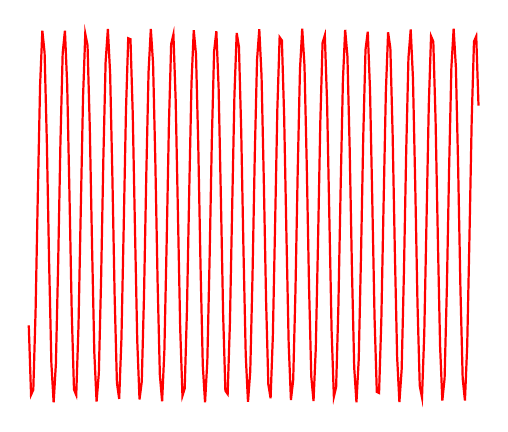
\begin{tikzpicture}
		\pgfmathdeclarefunction{S}{2}{\pgfmathparse{sin(deg(#1*#2*5.2))}}
	
		\begin{axis}
		[
		xtick={
			-6.28318, -4.7123889, -3.14159, -1.5708,
			1.5708, 3.14159, 4.7123889, 6.28318
		},
		xticklabels={
			$-2\pi$, $-\frac{3\pi}{2}$, $-\pi$, $\frac{\pi}{2}$,
			$\frac{\pi}{2}$, $\pi$, $\frac{3\pi}{2}$, $2\pi$
		},
		axis lines = none,
		grid=none,minor tick num=1,
		% xlabel=$x$,ylabel=$y$,
		tick align=inside,
		domain=-2*pi:2*pi,
		samples=200
		]
		\addplot [red,thick] {S(2,x)};
		\end{axis}
		\end{tikzpicture}
	}
	\caption{Ripples on a swimming pool}	
	\end{figure}
	
	You could also imagine in the same swimming pool on a calm day, a person could jump into the water creating waves that look similar to the ones below:
	
			\begin{figure}[h]
		\centering
		\resizebox{6in}{1in}{
			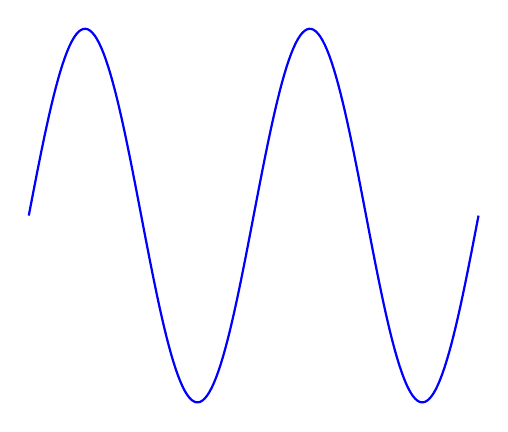
\begin{tikzpicture}
			\pgfmathdeclarefunction{S}{2}{\pgfmathparse{10*sin(deg(#1*#2/2))}}
			
			\begin{axis}
			[
			xtick={
				-6.28318, -4.7123889, -3.14159, -1.5708,
				1.5708, 3.14159, 4.7123889, 6.28318
			},
			xticklabels={
				$-2\pi$, $-\frac{3\pi}{2}$, $-\pi$, $\frac{\pi}{2}$,
				$\frac{\pi}{2}$, $\pi$, $\frac{3\pi}{2}$, $2\pi$
			},
			axis lines = none,
			grid=none,minor tick num=1,
			% xlabel=$x$,ylabel=$y$,
			tick align=inside,
			domain=-2*pi:2*pi,
			samples=200
			]
			\addplot [blue,thick] {S(2,x)};
			\end{axis}
			\end{tikzpicture}
		}
		
	\caption{Large waves in a swimming pool}
	\end{figure}


Thus, we can use the principle of superposition  to predict what the wave will look like should a person jump into the swimming pool on a day when there are ripples in the water.  By combining the two types of waves, we would see something like the figure below:

		\begin{figure}[h]
	\centering
	\resizebox{6in}{1in}{
		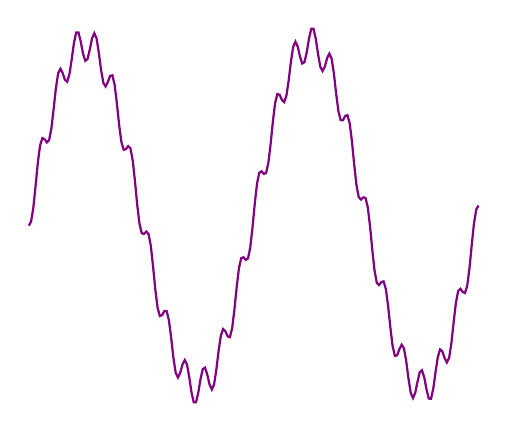
\begin{tikzpicture}
		\pgfmathdeclarefunction{S}{2}{\pgfmathparse{(sin(deg(#1*#2*6.2)))}}
			\pgfmathdeclarefunction{C}{2}{\pgfmathparse{10*sin(deg(#1*#2/2))}}
		
		\begin{axis}
		[
		xtick={
			-6.28318, -4.7123889, -3.14159, -1.5708,
			1.5708, 3.14159, 4.7123889, 6.28318
		},
		xticklabels={
			$-2\pi$, $-\frac{3\pi}{2}$, $-\pi$, $\frac{\pi}{2}$,
			$\frac{\pi}{2}$, $\pi$, $\frac{3\pi}{2}$, $2\pi$
		},
		axis lines = none,
		grid=none,minor tick num=1,
		% xlabel=$x$,ylabel=$y$,
		tick align=inside,
		domain=-2*pi:2*pi,
		samples=200
		]
		\addplot [violet,thick] {S(2,x)+C(2,x)};
		\end{axis}
		\end{tikzpicture}
	}
	
	\caption{Ripples and waves combine}
\end{figure}
















\newpage

\subsection{Interference}
\subsubsection{Constructive Interference}


Sometimes, waves of approximately the same amplitude may overlap, causing the amplitude of the resulting wave to become larger.  This is called \textbf{Constructive Interference}: \index{Interference, Constructive}
\begin{figure}[h]
\newcolumntype{C}{ >{\centering\arraybackslash} m{1.5in} }
\newcolumntype{D}{ >{\centering\arraybackslash} m{.25in} }
\begin{tabular}{C D C D C }
	
	\resizebox{1in}{.25in}{
		\begin{tikzpicture}
		\pgfmathdeclarefunction{S}{2}{\pgfmathparse{(sin(deg(#1*#2)))}}
		
		
		\begin{axis}
		[
		xtick={
			-6.28318, -4.7123889, -3.14159, -1.5708,
			1.5708, 3.14159, 4.7123889, 6.28318
		},
		xticklabels={
			$-2\pi$, $-\frac{3\pi}{2}$, $-\pi$, $\frac{\pi}{2}$,
			$\frac{\pi}{2}$, $\pi$, $\frac{3\pi}{2}$, $2\pi$
		},
		axis lines = none,
		grid=none,minor tick num=1,
		% xlabel=$x$,ylabel=$y$,
		tick align=inside,
		domain=0:pi,
		samples=200
		]
		\addplot [red,thick] {S(2,x)};
		\end{axis}
		\end{tikzpicture}
	}
	
	&
	+
	&
	
	\resizebox{1in}{.5in}{
		\begin{tikzpicture}
		\pgfmathdeclarefunction{S}{2}{\pgfmathparse{(sin(deg(#1*#2)))}}
		
		
		\begin{axis}
		[
		xtick={
			-6.28318, -4.7123889, -3.14159, -1.5708,
			1.5708, 3.14159, 4.7123889, 6.28318
		},
		xticklabels={
			$-2\pi$, $-\frac{3\pi}{2}$, $-\pi$, $\frac{\pi}{2}$,
			$\frac{\pi}{2}$, $\pi$, $\frac{3\pi}{2}$, $2\pi$
		},
		axis lines = none,
		grid=none,minor tick num=1,
		% xlabel=$x$,ylabel=$y$,
		tick align=inside,
		domain=0:pi,
		samples=200
		]
		\addplot [red,thick] {S(2,x)};
		\end{axis}
		\end{tikzpicture}
	}
	&
	$\longrightarrow$
	&
	
	\resizebox{1in}{.75in}{
		\begin{tikzpicture}
		\pgfmathdeclarefunction{S}{2}{\pgfmathparse{(sin(deg(#1*#2)))}}
		
		
		\begin{axis}
		[
		xtick={
			-6.28318, -4.7123889, -3.14159, -1.5708,
			1.5708, 3.14159, 4.7123889, 6.28318
		},
		xticklabels={
			$-2\pi$, $-\frac{3\pi}{2}$, $-\pi$, $\frac{\pi}{2}$,
			$\frac{\pi}{2}$, $\pi$, $\frac{3\pi}{2}$, $2\pi$
		},
		axis lines = none,
		grid=none,minor tick num=1,
		% xlabel=$x$,ylabel=$y$,
		tick align=inside,
		domain=0:pi,
		samples=200
		]
		\addplot [red,thick] {S(2,x)};
		\end{axis}
		\end{tikzpicture}
	}
\end{tabular}
\caption{Constructive interference}
\end{figure}

In order for constructive interference to happen, the two waves must be \textit{in phase} - that is, the displacement of the waves must be in the same direction. 


When two waves that are continuous overlap, they will interfere constructively if they align perfectly:


	
\begin{figure}[h]
	\centering

		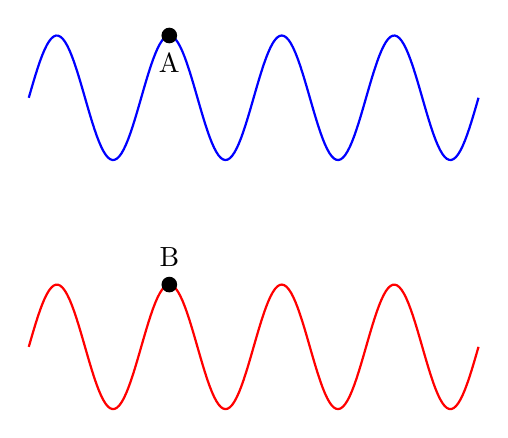
\begin{tikzpicture}
		\pgfmathdeclarefunction{S}{2}{\pgfmathparse{sin(deg(#1*#2))}}
		
		\begin{axis}
		[
		xtick={
			-6.28318, -4.7123889, -3.14159, -1.5708,
			1.5708, 3.14159, 4.7123889, 6.28318
		},
		xticklabels={
			$-2\pi$, $-\frac{3\pi}{2}$, $-\pi$, $\frac{\pi}{2}$,
			$\frac{\pi}{2}$, $\pi$, $\frac{3\pi}{2}$, $2\pi$
		},
		axis lines = none,
		grid=major, minor tick num=1,
		xticklabels={},yticklabels={},
		ymajorgrids=false,
		 xlabel=,ylabel=,
		tick align=inside,
		domain=-2*pi:2*pi,
		range=-1:8,
		samples=200
		]
		\addplot [red,thick] {S(2,x)};
		\addplot [blue,thick] {S(2,x)+4};
	\node[label=B,circle,fill, inner sep=2pt] at (axis cs:-2.35619449019,1) {};
	\node[label=below:{A},circle,fill, inner sep=2pt] at (axis cs:-2.35619449019,5) {};
		\end{axis}
	
		
		\end{tikzpicture}
	
	\caption{Two waves aligned perfectly}	
	
\end{figure}


Likewise, constructive interference will occur if the wave is shifted by a distance of one wavelength.  


\begin{figure}[h]
	\centering
	
	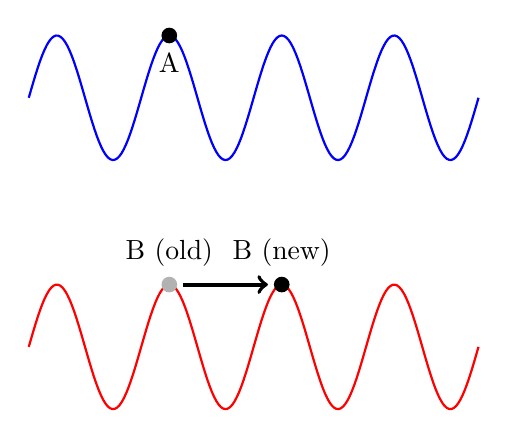
\begin{tikzpicture}
	\pgfmathdeclarefunction{S}{2}{\pgfmathparse{sin(deg(#1*#2))}}
	
	\begin{axis}
	[
	xtick={
		-6.28318, -4.7123889, -3.14159, -1.5708,
		1.5708, 3.14159, 4.7123889, 6.28318
	},
	xticklabels={
		$-2\pi$, $-\frac{3\pi}{2}$, $-\pi$, $\frac{\pi}{2}$,
		$\frac{\pi}{2}$, $\pi$, $\frac{3\pi}{2}$, $2\pi$
	},
	axis lines = none,
	grid=major, minor tick num=1,
	xticklabels={},yticklabels={},
	ymajorgrids=false,
	xlabel=,ylabel=,
	tick align=inside,
	domain=-2*pi:2*pi,
	range=-1:8,
	samples=200
	]
	\addplot [red,thick] {S(2,x)};
	\addplot [blue,thick] {S(2,x)+4};
	\node[label={B (old)},circle,fill=black!30!white, inner sep=2pt] at (axis cs:-2.35619449019,1) {};
	\node[label={B (new)},circle,fill, inner sep=2pt] at (axis cs:0.785398,1) {};
	\node[label=below:{A},circle,fill, inner sep=2pt] at (axis cs:-2.35619449019,5) {};
	\coordinate [label={}]  (A) at (-2.35619449019,1)  ;
	\coordinate [label={}]  (B) at (0.785398,1) ;
	\draw [->,line width=0.5mm, black ,shorten <= 5pt, shorten >= 5pt](A) -- (B) ;
	
	
	
	\end{axis}
	
	
	\end{tikzpicture}
	
	\caption{The red wave has been shifted one wavelength to the right.}	
	
\end{figure}

The wave could be shifted in a similar manner by two, three, or any integer number of wavelengths right or left, and the two waves will still cause constructive interference.  Thus, the amount of shift between the waves, $\Delta \ell$, is given by:


	
\begin{mdframed}[backgroundcolor=orange!20!white]
	\begin{equation}
	\Delta \ell = m \lambda
	\label{equation:constructiveinterference}
	\end{equation}
\end{mdframed}	

where $\Delta \ell$ is how far the waves are shifted, and $m$ is any integer.








\subsubsection{Destructive Interference}

	At other times, waves may overlap while they are \textbf{out of phase} - that is, their displacement is in opposite directions, causing the wave to become smaller. This is called \textbf{destructive interference}.   \index{Interference, Destructive}

	
	\begin{figure}[h]
		\newcolumntype{C}{ >{\centering\arraybackslash} m{1.5in} }
		\newcolumntype{D}{ >{\centering\arraybackslash} m{.25in} }
		\begin{tabular}{C D C D C }
			
			\resizebox{1in}{.75in}{
				\begin{tikzpicture}
				\pgfmathdeclarefunction{S}{2}{\pgfmathparse{(sin(deg(#1*#2)))}}
				
				
				\begin{axis}
				[
				xtick={
					-6.28318, -4.7123889, -3.14159, -1.5708,
					1.5708, 3.14159, 4.7123889, 6.28318
				},
				xticklabels={
					$-2\pi$, $-\frac{3\pi}{2}$, $-\pi$, $\frac{\pi}{2}$,
					$\frac{\pi}{2}$, $\pi$, $\frac{3\pi}{2}$, $2\pi$
				},
				axis lines = none,
				grid=none,minor tick num=1,
				% xlabel=$x$,ylabel=$y$,
				tick align=inside,
				domain=0:pi,
				samples=200
				]
				\addplot [red,thick] {S(2,x)};
				\end{axis}
				\end{tikzpicture}
			}
			
			&
			+
			&
			
			\resizebox{1in}{1in}{
				\begin{tikzpicture}
				\pgfmathdeclarefunction{S}{2}{\pgfmathparse{(sin(deg(#1*#2)))}}
				
				
				\begin{axis}
				[
				xtick={
					-6.28318, -4.7123889, -3.14159, -1.5708,
					1.5708, 3.14159, 4.7123889, 6.28318
				},
				xticklabels={
					$-2\pi$, $-\frac{3\pi}{2}$, $-\pi$, $\frac{\pi}{2}$,
					$\frac{\pi}{2}$, $\pi$, $\frac{3\pi}{2}$, $2\pi$
				},
				axis lines = none,
				grid=none,minor tick num=1,
				% xlabel=$x$,ylabel=$y$,
				tick align=inside,
				domain=0:pi,
				samples=200
				]
				\addplot [red,thick] {-S(2,x)};
				\end{axis}
				\end{tikzpicture}
			}
			&
			$\longrightarrow$
			&
			
			\resizebox{1in}{.25in}{
				\begin{tikzpicture}
				\pgfmathdeclarefunction{S}{2}{\pgfmathparse{(sin(deg(#1*#2)))}}
				
				
				\begin{axis}
				[
				xtick={
					-6.28318, -4.7123889, -3.14159, -1.5708,
					1.5708, 3.14159, 4.7123889, 6.28318
				},
				xticklabels={
					$-2\pi$, $-\frac{3\pi}{2}$, $-\pi$, $\frac{\pi}{2}$,
					$\frac{\pi}{2}$, $\pi$, $\frac{3\pi}{2}$, $2\pi$
				},
				axis lines = none,
				grid=none,minor tick num=1,
				% xlabel=$x$,ylabel=$y$,
				tick align=inside,
				domain=0:pi,
				samples=200
				]
				\addplot [red,thick] {-S(2,x)};
				\end{axis}
				\end{tikzpicture}
			}
		\end{tabular}
		\caption{Destructive Interference}
	\end{figure}
	
	
	
	
	If two waves are displaced by the same amount in opposite directions, they can even cancel out completely.  This would be \textbf{perfectly destructive interference}: 
	
		\begin{figure}[h]
		\newcolumntype{C}{ >{\centering\arraybackslash} m{1.5in} }
		\newcolumntype{D}{ >{\centering\arraybackslash} m{.25in} }
		\begin{tabular}{C D C D C }
			
			\resizebox{1in}{1in}{
				\begin{tikzpicture}
				\pgfmathdeclarefunction{S}{2}{\pgfmathparse{(sin(deg(#1*#2)))}}
				
				
				\begin{axis}
				[
				xtick={
					-6.28318, -4.7123889, -3.14159, -1.5708,
					1.5708, 3.14159, 4.7123889, 6.28318
				},
				xticklabels={
					$-2\pi$, $-\frac{3\pi}{2}$, $-\pi$, $\frac{\pi}{2}$,
					$\frac{\pi}{2}$, $\pi$, $\frac{3\pi}{2}$, $2\pi$
				},
				axis lines = none,
				grid=none,minor tick num=1,
				% xlabel=$x$,ylabel=$y$,
				tick align=inside,
				domain=0:pi,
				samples=200
				]
				\addplot [red,thick] {S(2,x)};
				\end{axis}
				\end{tikzpicture}
			}
			
			&
			+
			&
			
			\resizebox{1in}{1in}{
				\begin{tikzpicture}
				\pgfmathdeclarefunction{S}{2}{\pgfmathparse{(sin(deg(#1*#2)))}}
				
				
				\begin{axis}
				[
				xtick={
					-6.28318, -4.7123889, -3.14159, -1.5708,
					1.5708, 3.14159, 4.7123889, 6.28318
				},
				xticklabels={
					$-2\pi$, $-\frac{3\pi}{2}$, $-\pi$, $\frac{\pi}{2}$,
					$\frac{\pi}{2}$, $\pi$, $\frac{3\pi}{2}$, $2\pi$
				},
				axis lines = none,
				grid=none,minor tick num=1,
				% xlabel=$x$,ylabel=$y$,
				tick align=inside,
				domain=0:pi,
				samples=200
				]
				\addplot [red,thick] {-S(2,x)};
				\end{axis}
				\end{tikzpicture}
			}
			&
			$\longrightarrow$
			&
			
			\resizebox{1in}{.01in}{
				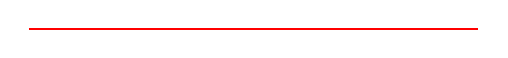
\begin{tikzpicture}
				\pgfmathdeclarefunction{S}{2}{\pgfmathparse{(sin(deg(#1*#2)))}}
				
				
				\begin{axis}
				[
				xtick={
					-6.28318, -4.7123889, -3.14159, -1.5708,
					1.5708, 3.14159, 4.7123889, 6.28318
				},
				xticklabels={
					$-2\pi$, $-\frac{3\pi}{2}$, $-\pi$, $\frac{\pi}{2}$,
					$\frac{\pi}{2}$, $\pi$, $\frac{3\pi}{2}$, $2\pi$
				},
				axis lines = none,
				grid=none,minor tick num=1,
				% xlabel=$x$,ylabel=$y$,
				tick align=inside,
				domain=0:pi,
				samples=200
				]
				\addplot [red,thick] {0 * S(2,x)};
				\end{axis}
				\end{tikzpicture}
			}
		\end{tabular}
		\caption{Perfectly Destructive Interference}
	\end{figure}
		\newpage 
	
	In order for destructive interference to happen, the two waves must be perfectly \textit{out of phase} - that is, the displacement of the waves must be in opposite direction, meaning the waves are already shifted by a half wavelength:
	
	
	
	\begin{figure}[h]
		\centering
		
		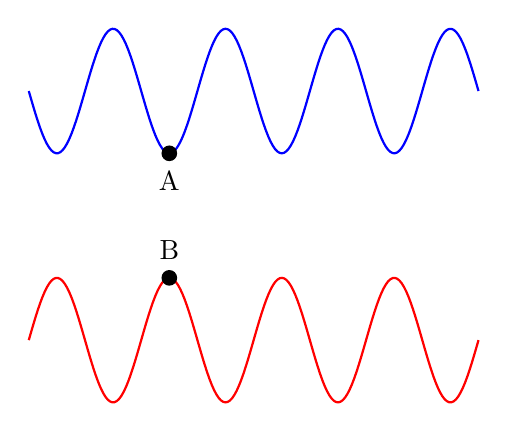
\begin{tikzpicture}
		\pgfmathdeclarefunction{S}{2}{\pgfmathparse{sin(deg(#1*#2))}}
		
		\begin{axis}
		[
		xtick={
			-6.28318, -4.7123889, -3.14159, -1.5708,
			1.5708, 3.14159, 4.7123889, 6.28318
		},
		xticklabels={
			$-2\pi$, $-\frac{3\pi}{2}$, $-\pi$, $\frac{\pi}{2}$,
			$\frac{\pi}{2}$, $\pi$, $\frac{3\pi}{2}$, $2\pi$
		},
		axis lines = none,
		grid=major, minor tick num=1,
		xticklabels={},yticklabels={},
		ymajorgrids=false,
		xlabel=,ylabel=,
		tick align=inside,
		domain=-2*pi:2*pi,
		range=-1:8,
		samples=200
		]
		\addplot [red,thick] {S(2,x)};
		\addplot [blue,thick] {S(2,x+1.5708)+4};
		\node[label=B,circle,fill, inner sep=2pt] at (axis cs:-2.35619449019,1) {};
		\node[label=below:{A},circle,fill, inner sep=2pt] at (axis cs:-2.35619449019,3) {};
		\end{axis}
		
		
		\end{tikzpicture}
		
		\caption{Two waves aligned perfectly}	
		
	\end{figure}
	
	
		
		
	Likewise, destructive interference will occur if the wave is shifted by a distance of one wavelength (after already being off by half a wavelength).  
	

	
	\begin{figure}[!h]
		\centering
		
		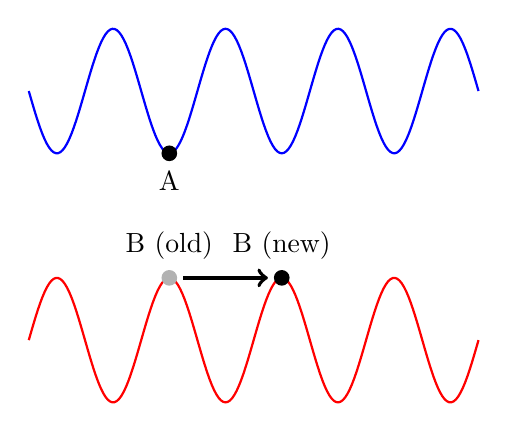
\begin{tikzpicture}
		\pgfmathdeclarefunction{S}{2}{\pgfmathparse{sin(deg(#1*#2))}}
		
		\begin{axis}
		[
		xtick={
			-6.28318, -4.7123889, -3.14159, -1.5708,
			1.5708, 3.14159, 4.7123889, 6.28318
		},
		xticklabels={
			$-2\pi$, $-\frac{3\pi}{2}$, $-\pi$, $\frac{\pi}{2}$,
			$\frac{\pi}{2}$, $\pi$, $\frac{3\pi}{2}$, $2\pi$
		},
		axis lines = none,
		grid=major, minor tick num=1,
		xticklabels={},yticklabels={},
		ymajorgrids=false,
		xlabel=,ylabel=,
		tick align=inside,
		domain=-2*pi:2*pi,
		range=-1:8,
		samples=200
		]
		\addplot [red,thick] {S(2,x)};
		\addplot [blue,thick] {S(2,x+1.5708)+4};
		\node[label={B (old)},circle,fill=black!30!white, inner sep=2pt] at (axis cs:-2.35619449019,1) {};
		\node[label={B (new)},circle,fill, inner sep=2pt] at (axis cs:0.785398,1) {};
		\node[label=below:{A},circle,fill, inner sep=2pt] at (axis cs:-2.35619449019,3) {};
		\coordinate [label={}]  (A) at (-2.35619449019,1)  ;
		\coordinate [label={}]  (B) at (0.785398,1) ;
		\draw [->,line width=0.5mm, black ,shorten <= 5pt, shorten >= 5pt](A) -- (B) ;
		
		
		
		\end{axis}
		
		
		\end{tikzpicture}
		
		\caption{The red wave has been shifted one wavelength to the right.}	
		
	\end{figure}
	
	Since destructive interference occurs whenever the waves are shifted by half-integer multiples of the wavelength (ie, 0.5, 1.5, 2.5, etc), the amount of shift between the waves, $\Delta \ell$, is given by:
	
	
	
	\begin{mdframed}[backgroundcolor=orange!20!white]
		\begin{equation}
		\Delta \ell = (m+\frac{1}{2}) \lambda
		\label{equation:destructiveinterference}
		\end{equation}
	\end{mdframed}	
	
	where $\Delta \ell$ is how far the waves are shifted, and $m$ is any integer.
	
	\newpage 
	
	
	\begin{mdframed}[backgroundcolor=blue!10!white]
		\begin{center}
			
			
			\textbf{Example \thesection.1}	
		\end{center}
		
		\textbf{Problem: } Two trombone players stand in a single file line, with their conductor directly in front of them, as shown in the diagram: 
		
		\begin{center}
			\begin{tabular}{c c c c}
				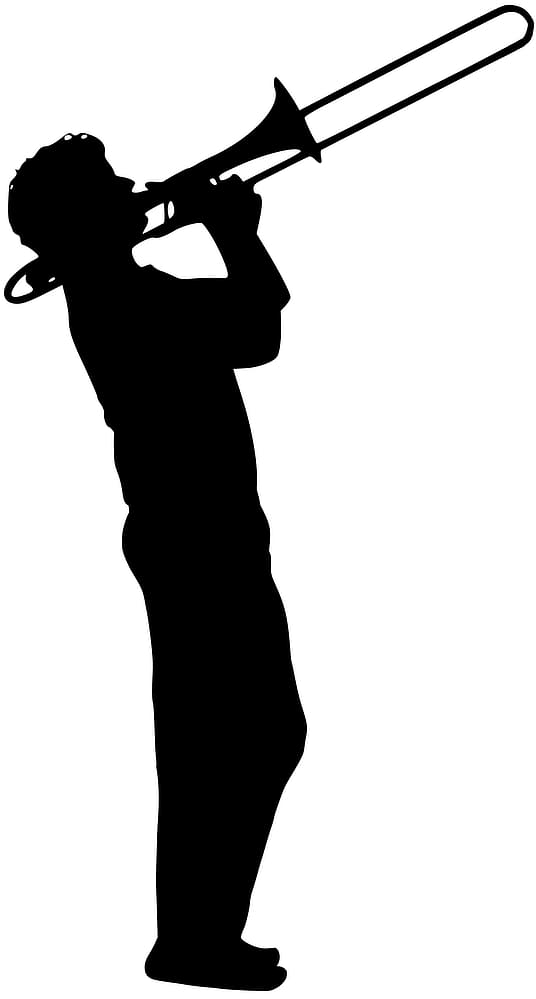
\includegraphics[height=0.75in]{Chapters/Ch10-Waves/trombone.png} & 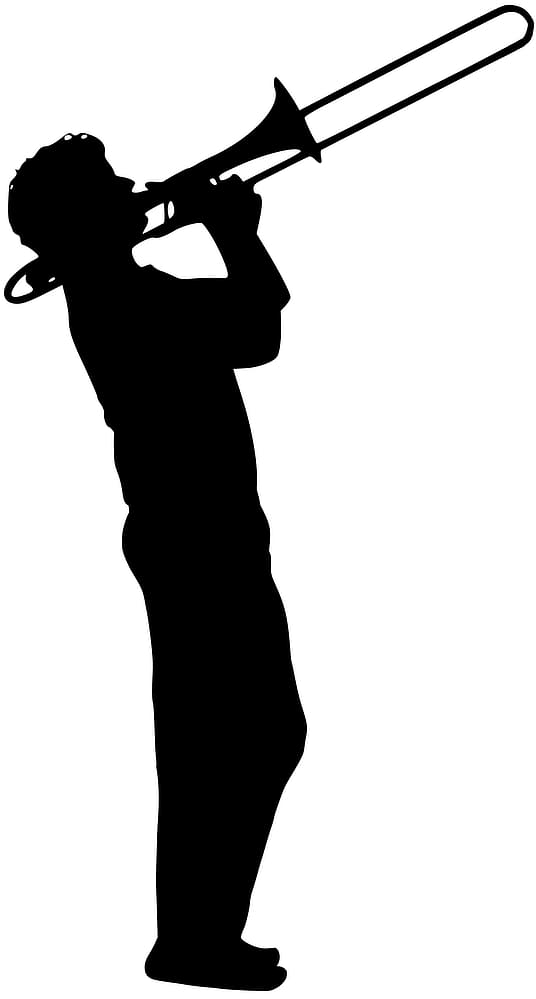
\includegraphics[height=0.75in]{Chapters/Ch10-Waves/trombone.png} & &
				
\includegraphics[height=0.75in]{Chapters/Ch10-Waves/conductor.png}
			\end{tabular}
		\end{center}
		\vspace{0.2in}
		Both trombones play a low-$B \flat$ ($f = \SI{116.54}{\Hz}$).  What is the smallest, non-zero distance that the players should stand apart in order for the conductor to hear the loudest possible sound?  (Assume both players are perfectly in tune and the waves they create are perfectly in phase.)
		
		
		
		
		
		\textbf{Solution:} 
		We already know:
		\begin{center}
			$f = \SI{116.54}{\Hz}$
			
			$v = \SI[per-mode = symbol]{343}{\m\per\s}$
		\end{center}
		Thus, we can use equation \ref{equation:wavevelocity} to find the wavelength:
		
		\begin{equation*}
		v = f \lambda \longrightarrow \lambda = \frac{v}{f} = \frac{\SI[per-mode = symbol]{343}{\m\per\s}}{\SI{116.54}{\Hz}} \approx {\SI{2.943}{\m}} 
		\end{equation*}
		
	Since we are asked for the loudest sound, we know that this is constructive interference. We know that if $m=0$, the distance between the two players will be zero.  Thus, the smallest non-zero distance is given when $m=1$.  Using equation \ref{equation:constructiveinterference}, we find:
		
		\begin{equation*}
			\Delta \ell = m \lambda = (1)(\SI{2.943}{m}) = \SI{2.943}{m}
		\end{equation*}		
	\end{mdframed}
	
	
	
	
	
	
	
	
	
	
	
	
	
	
	
	
	
	
	
		\newpage
	
	
\begin{mdframed}[backgroundcolor=blue!10!white]
		\begin{center}
			
			
			\textbf{Example \thesection.2}	
		\end{center}
		
		\textbf{Problem: } Two speakers are aligned along an east-west line, and are placed 1 meter apart.  A single frequency is played on both speakers.  A person starts in front of the left-most speaker, and begins to walk to the south.  When the person has walked 2 meters to the south, she hears the sound get significantly quieter.  As she continues to walk, he hears the sound get louder again.  What is the frequency of the sound?
		\vspace{0.2in}
		

		
	
		
		\textbf{Solution:} 
		Begin by drawing a diagram of the situation: 
		
		\begin{center}
		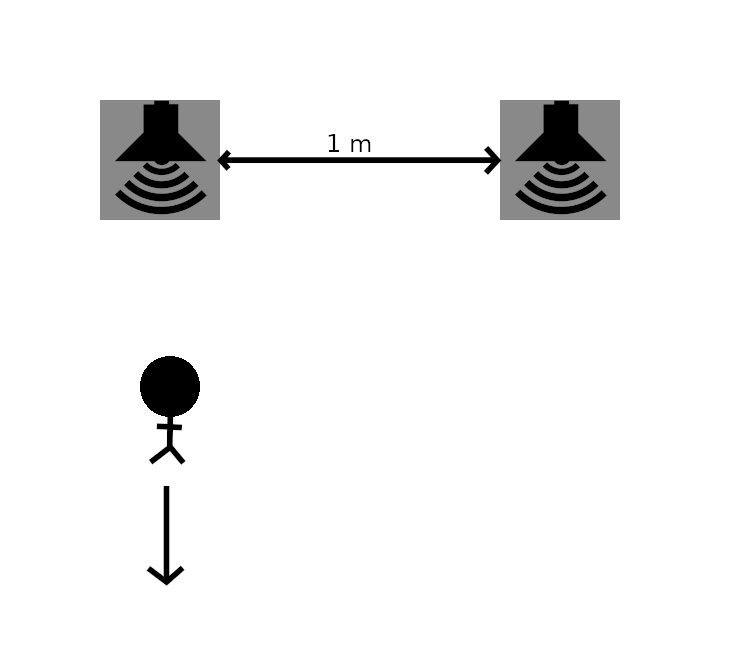
\includegraphics[height=1.5 in]{Chapters/Ch10-Waves/speakers.png}
		\end{center}
	
		We begin by calculating the difference in distances between the speakers.  The distance to the west speaker is 2 meters.  The distance to the right speaker can be found using the Pythagorean Theorem:
		
		\begin{equation*}
		c = \sqrt{a^2 + b^2} = \sqrt{(\SI{2}{\m})^2 + (\SI{1}{\m})^2} = \sqrt{\SI{5}{\m^2 }} \approx \SI{2.236}{\m}
		\end{equation*}
		
		Therefore, $\Delta \ell$, the distance between the two paths the sound is traveling is given by: 
		
		\begin{equation*}
		\Delta \ell = \SI{2.236}{\m} - \SI{2}{\m} \approx \SI{0.236}{\m}
		\end{equation*}
	
		Since this problem states that sound gets quieter, we know that this is destructive interference, and we can use equation \ref{equation:destructiveinterference}:  
		\begin{equation*}
		\Delta \ell = (m+\frac{1}{2}) \lambda
		\end{equation*}
		
		We know that the smallest value $m$ can be is 0, so our equation reduces to:
				
		\begin{equation*}
		\Delta \ell = (\cancelto{0}{m}+\frac{1}{2}) \lambda \longrightarrow \Delta \ell = \frac{\lambda}{2}
		\end{equation*}
		
		


		Solving for $\lambda$ gives:
		
		
		\begin{equation*}
		\lambda = 2 \Delta \ell = (2)(\SI{0.236}{\m}) = \SI{0.472}{\m}
		\end{equation*}
		
	
		Knowing that the speed of sound is 343 m/s, we can use equation \ref{equation:wavevelocity} to determine the frequency:
		
		\begin{equation*}
		v = f \lambda \longrightarrow f = \frac{v}{\lambda} = \frac{\SI[per-mode = symbol]{343}{\m\per\s}}{\SI{0.472}{m}} = \boxed{\SI{726.540}{\Hz}} 
		\end{equation*}
		

		 
	
		
	\end{mdframed}
	
	
	\section{Resonance}
	\index{Resonance}
	\textbf{Resonance} is a process in which waves reinforce each other through constructive interference, resulting a wave with much greater amplitude than the original wave.  
	
	\subsection{Resonance of a Tube that is Open on Both Ends}
	\subsection{Resonance of a Tube that is Open on One End and Closed on the Other}
	\subsection{Resonance of a String that is Fixed on Both Ends}
	
	
	
	
	

	
	
	

	

	


